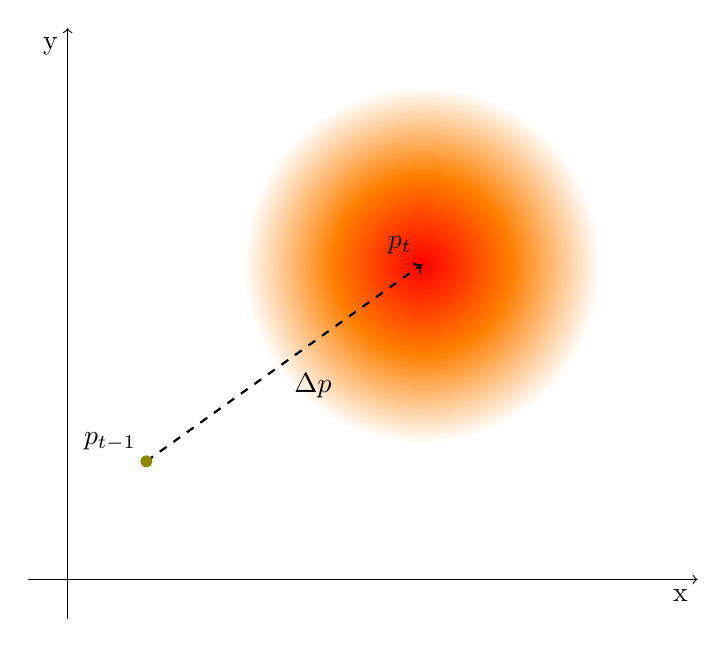
\begin{tikzpicture}
  % shading
  \pgfdeclareradialshading{ring}{\pgfpoint{0cm}{0cm}}%
  { %
    rgb(  0cm)=(1,0,0);
    rgb( .4cm)=(1,.5,0);
    rgb( .8cm)=(1,1,1);
    rgb(1.0cm)=(1,1,1)%;
  }

  % old and new pos
  \coordinate (oldPos) at(1,1.5);
  \coordinate (newPos) at(4.5,4);
  \coordinate (offset) at(.4,-.5);
  %\coordinate (deltaStart) at($(oldPos)+(offset)$);
  %\coordinate (deltaEnd)   at($(newPos)+(offset)$);

  % uncertainty
  \shade[shading=ring] (newPos) circle (2.5);

  % movement
  \draw[thick,dashed,->] (oldPos) node[above left]  {$p_{t-1}$} 
                              --  node[below right] {$\Delta p$} 
                         (newPos) node[above left]  {$p_{t}$};
  %\draw[thin,|-|] (deltaStart) --  (deltaEnd);

  % certain old pos
  \fill[olive] (oldPos) circle (.075);

  % axes
  \draw[thin, <->] (8,0) node[below left]{x} -| (0, 7) node[below left]{y};
  \draw[thin, -] (-0.5,0) -| (0,-0.5);
\end{tikzpicture}
